\chapter{Experiments}

\section{AE vs VAE}

As described in previous sections, our main goal is to create an end-to-end RL algorithm composed of an encoder followed by SAC. To determine whether to use an AutoEncoder or a Variational AutoEncoder we investigate if the stochasticity of VAEs can help in learning a good representation of the actual state. 

In order to chose which architecture to use, we train an AE where the encoder is composed of 3 sequential convolutional linear layers interposed by a ReLU function and on output layer of size to be defined, similarly the decoder is composed of 3 deconvolutional layers. The VAE, instead, is composed of 4 convolutional/deconvolutional layers. The detailed architecture can be found in APPENDIX \ref{app:ae/vae}. Each network has been trained for 50 epochs on our training set with an early stopping on the fifth contiguous epoch with no improvement on the validation loss.

The latent size ($z\_size$) must be carefully chosen such that the latent space is able to represent all the features extracted from the images and consequently produce high quality reconstruction. In particular, our tests plan to use 32 and 64 dimensional latent spaces. 

To further improve the generalization of our encoders and the robustness of our learned representation, image augmentation is a suitable technique. In particular, we consider several augmentation methods such as Gaussian and motion blurring, contrast normalization, additive Gaussian noise, sharpening and coarse dropout. In training each images can be randomly augmented by some of the aforementioned transformation. 

Each of the architecture with the different $z\_size$ and with augmentation enabled or disabled is then trained three time for each of the training set (simulated and real), and the results are averaged to increase to reliability. 

After the training, each model is evaluated on the test set and the resulting reconstruction loss (MSE) are averaged to identify which is the absolute best encoder. 

The results reported in Tables \ref{tab:aesim}-\ref{tab:vaereal} clearly shown how, in all cases, each encoder obtains lower reconstruction loss mean when augmentation is disabled since its activation causes early stopping in all tested case. A further contribution to the reduction of the loss is given by a bigger latent space, in fact, in all cases, the encoder with a latent space of 64 dimension performs better. Finally, our VAEs outperform significantly all the AEs, that is why we will use them to carry out all the next experiments, both in real world and in simulation.
As described above, those pre-trained VAEs will remain unchanged for the entire duration of the RL agent training that follow. 

In Figures \ref{fig:realvaeexample} and \ref{fig:simvaeexample} is shown an example of what are the capabilities of the chosen VAEs in terms of reconstruction. From now on we will refer to the VAE trained on the dataset of pictures collected in the simulator with the name \textit{simulated VAE} and to the one trained on pictures collected in the real world with name \textit{real VAE} for simplicity. 


\begin{figure}[h]
  \begin{minipage}{.50\textwidth}
    \centering
    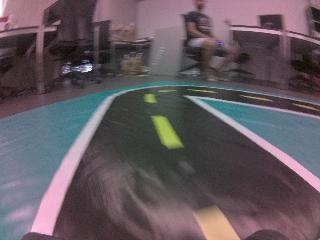
\includegraphics[height=0.50\textwidth]{experiments/11296.jpg}
  \end{minipage}%
  \begin{minipage}{.50\textwidth}
      \centering
      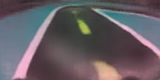
\includegraphics[width=0.60\textwidth]{experiments/11296.png}
  \end{minipage}
  \captionof{figure}{On the left an image from the real world as seen by the DonkeyCar camera, on the right the encoded and reconstructed image by the chosen VAE with a reconstruction loss of 112.}
  \label{fig:realvaeexample}
% \end{figure}
% \begin{figure}
  \begin{minipage}{.50\textwidth}
    \centering
    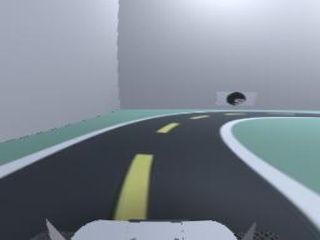
\includegraphics[height=0.50\textwidth]{experiments/1160.jpg}
  \end{minipage}%
  \begin{minipage}{.50\textwidth}
      \centering
      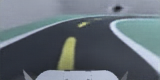
\includegraphics[width=0.60\textwidth]{experiments/1160.png}
  \end{minipage}
  \captionof{figure}{On the left an image from the simulator as seen by the DonkeyCar camera, on the right the encoded and reconstructed image by the chosen VAE with a reconstruction loss of 17}
  \label{fig:simvaeexample}
\end{figure}

\begin{table}[h]
  \centering
  \begin{tabular}{|c|c||c|c|c|c|}
  \hline
  Z\_SIZE & AUGMENTATION & MEAN & STD & MAX & MIN \\ \hline
  \multirow{2}{*}{32} & False & 121.54 & 102.42 & 795.44 & 45.61 \\
  & True & 164.57 & 95.51 & 783.03 & 65.13  \\ \hline
  \multirow{2}{*}{64} & False & 103.54 & 79.14 & 588.14 & 40.84 \\
  & True & 137.24 & 74,02 & 611,81 & 63,05  \\ \hline
  \end{tabular}
  \caption{AE trained in simulation - reconstruction loss}
  \label{tab:aesim}

  \begin{tabular}{|c|c||c|c|c|c|}
  \hline
  Z\_SIZE & AUGMENTATION & MEAN & STD & MAX & MIN \\ \hline
  \multirow{2}{*}{32} & False & 377.07 & 87.53 & 756.7 & 239.46 \\
  & True & 493.84 & 99.40 & 807.67 & 289.99  \\ \hline
  \multirow{2}{*}{64} & False & 311.1 & 78.5 & 695.65 & 177.77 \\
  & True & 411.37 & 77.30 & 647.68 & 241.87 \\ \hline
  \end{tabular}
  \caption{AE trained in real world - reconstruction loss}
  \label{tab:aereal}

  \begin{tabular}{|c|c||c|c|c|c|}
  \hline
  Z\_SIZE & AUGMENTATION & MEAN & STD & MAX & MIN \\ \hline
  \multirow{2}{*}{32} & False & 59.1 & 60.41 & 620.93 & 18.88 \\
  & True & 116.31 & 71.11 & 771.88 & 51.10  \\ \hline
  \multirow{2}{*}{64} & False & 45.15 & 43.49 & 480.22 & 14.34 \\
  & True & 112.17 & 59.79 & 573.19 & 54.28  \\ \hline
  \end{tabular}
  \caption{VAE trained in simulation - reconstruction loss}
  \label{tab:vaesim}

  \begin{tabular}{|c|c||c|c|c|c|}
  \hline
  Z\_SIZE & AUGMENTATION & MEAN & STD & MAX & MIN \\ \hline
  \multirow{2}{*}{32} & False & 227.4 & 44.74 & 418.7 & 140.12 \\
  & True & 263.87 & 52.29 & 478.26 & 172.70 \\ \hline
  \multirow{2}{*}{64} & False & 184.56 & 36.86 & 347.59 & 96.7 \\
  & True & 230.66 & 42.24 & 402.67 & 156.61  \\ \hline
  \end{tabular}
  \caption{VAE trained in real world - reconstruction loss}
  \label{tab:vaereal}
\end{table}

\section{RL algorithm}

\subsection{Reward function}
Designing a reward function that can work in both simulated and real environments is not trivial given the fundamental differences between them. In simulation, for example, the environment can provide supervision and useful information such as the position of the car and the speed. In our real setup, instead, the DonkeyCar can only leverage information coming through the camera frames. The reward function designed to work in simulation consists of four parts. The first one is a single point gained by the agent for every step made, intending to improve the length of the path as much as possible. Secondly, a throttle reward term increases the reward by a value proportional to the throttle to encourage the agent to drive as fast as possible. Moreover, a cross-track error penalty is proportional to the distance of the car from the center of the roadway that disincentives the agent as soon as it moves away from the center. Finally, as soon as the agent crashes or exceeds the maximum cross-track error allowed a big penalty is given. Thus, the reward function to be maximized is composed as follows:

\begin{equation}
  \label{eq:stdreward}
    r_t = 1 + throttle\_reward + cte\_penalty + \left\{\begin{matrix}
    if done & crash\_error \\ 
    else & 0  
    \end{matrix}\right.
\end{equation}
In our setup, the throttle is kept constant for the purposes of this thesis.
The reward function described above is used to test our simulated algorithm and as a starting point, however, we need to adapt it such that it can work also in the real world where the cross-track error is not available. To tackle the issue we simply remove the CTE penalty, even though this will lead to a major problem of shaky motion as described in the next section. The final reward function that has proven to work in both environments and that we will use in the following training procedures is computed as follows:
\begin{equation}
  \label{eq:realreward}
    r_t = 1 + throttle\_reward + \left\{\begin{matrix}
    if done & crash\_error \\ 
    else & 0  
    \end{matrix}\right.
\end{equation}
Since we want real and simulated version of our agent as similar as possible, Equation \ref{eq:realreward} is finally used in both cases.

\subsection{Training the simulated RL agent}
As a baseline for our RL algorithm, we used the source code provided by \citet{learning-to-drive-in-5-minutes} as a baseline. His algorithm allows the training of many RL algorithms, including the SAC of our interest, of both simulated and real-world agents, however, training on simulation with communication being over the internet is more computationally expensive and more prone to errors. Thus, for the simulation, we refactor the algorithm such that the communication happens locally. Moreover, his algorithm uses an AE which needs to be changed with the more performant VAE chosen above. To train our agents, we need to define what is the best strategy in terms of the starting point. We identified four main options, the first one lets the Donkey start always at the starting line, the second option starts the Donkey from a random checkpoint, the third one at the latest checkpoint reached in the previous episode and finally, the last option makes it start from all checkpoints cyclically. Defining in simulation which is the best strategy can save computational time in real-world training. To identify which one eventually converges more quickly and if it does, 4 different agents were trained, one for each option aforementioned. The quality measures to evaluate the trained agents, illustrated below in Figure \ref{fig:agentresults}, are the \textit{Episode success rate} that shows how many laps have been completed on average during the training, the \textit{Episode Reward mean} and the \textit{Episode Length mean}. All the models have been trained for 100k iterations which correspond to $\approx 2$ hours of training. \textit{ Agent 1} started each lap at a random checkpoint,\textit{ Agent 2} started always at the starting line,\textit{ Agent 3} at the latest checkpoint reached during the last episode, and, finally,\textit{ Agent 4} cyclically uses all the checkpoints.
\begin{figure}[h]
  \centering
  \begin{subfigure}{.45\linewidth}
      \centering
      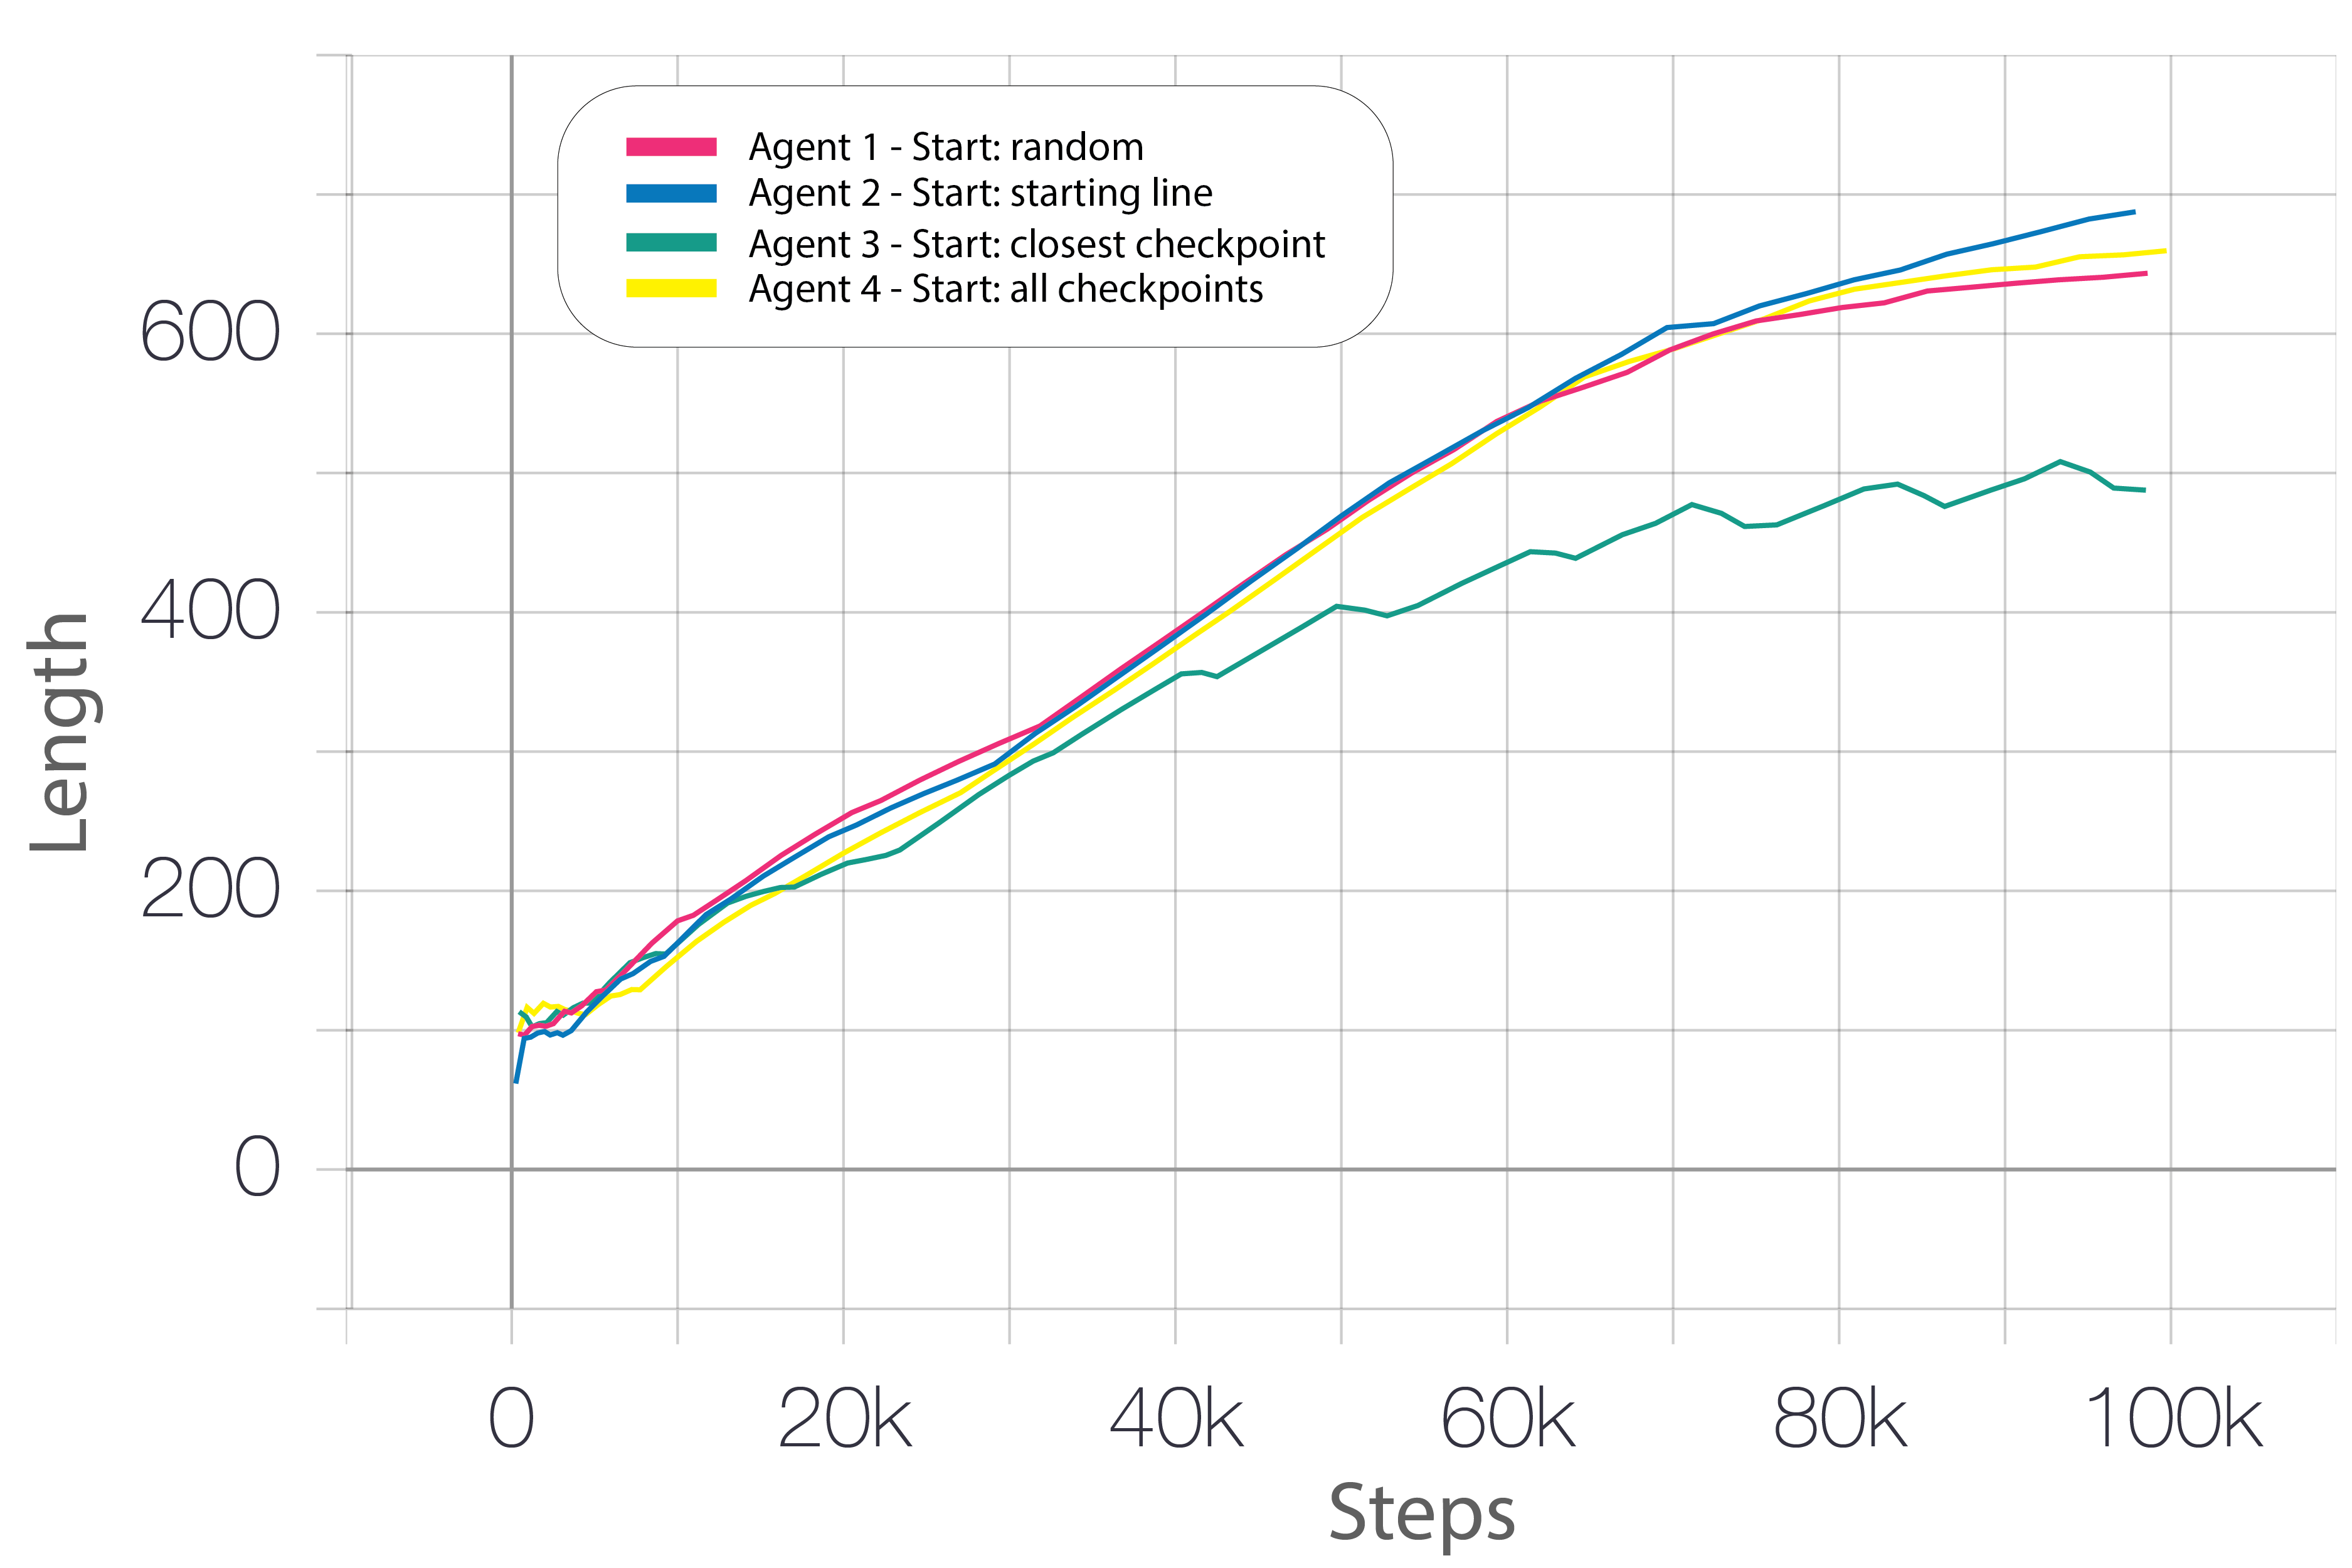
\includegraphics[width=1\textwidth]{experiments/len_mean.png}
      \caption{Episodes length mean}\label{fig:len}
  \end{subfigure}%
      \hfill
  \begin{subfigure}{.45\linewidth}
      \centering
      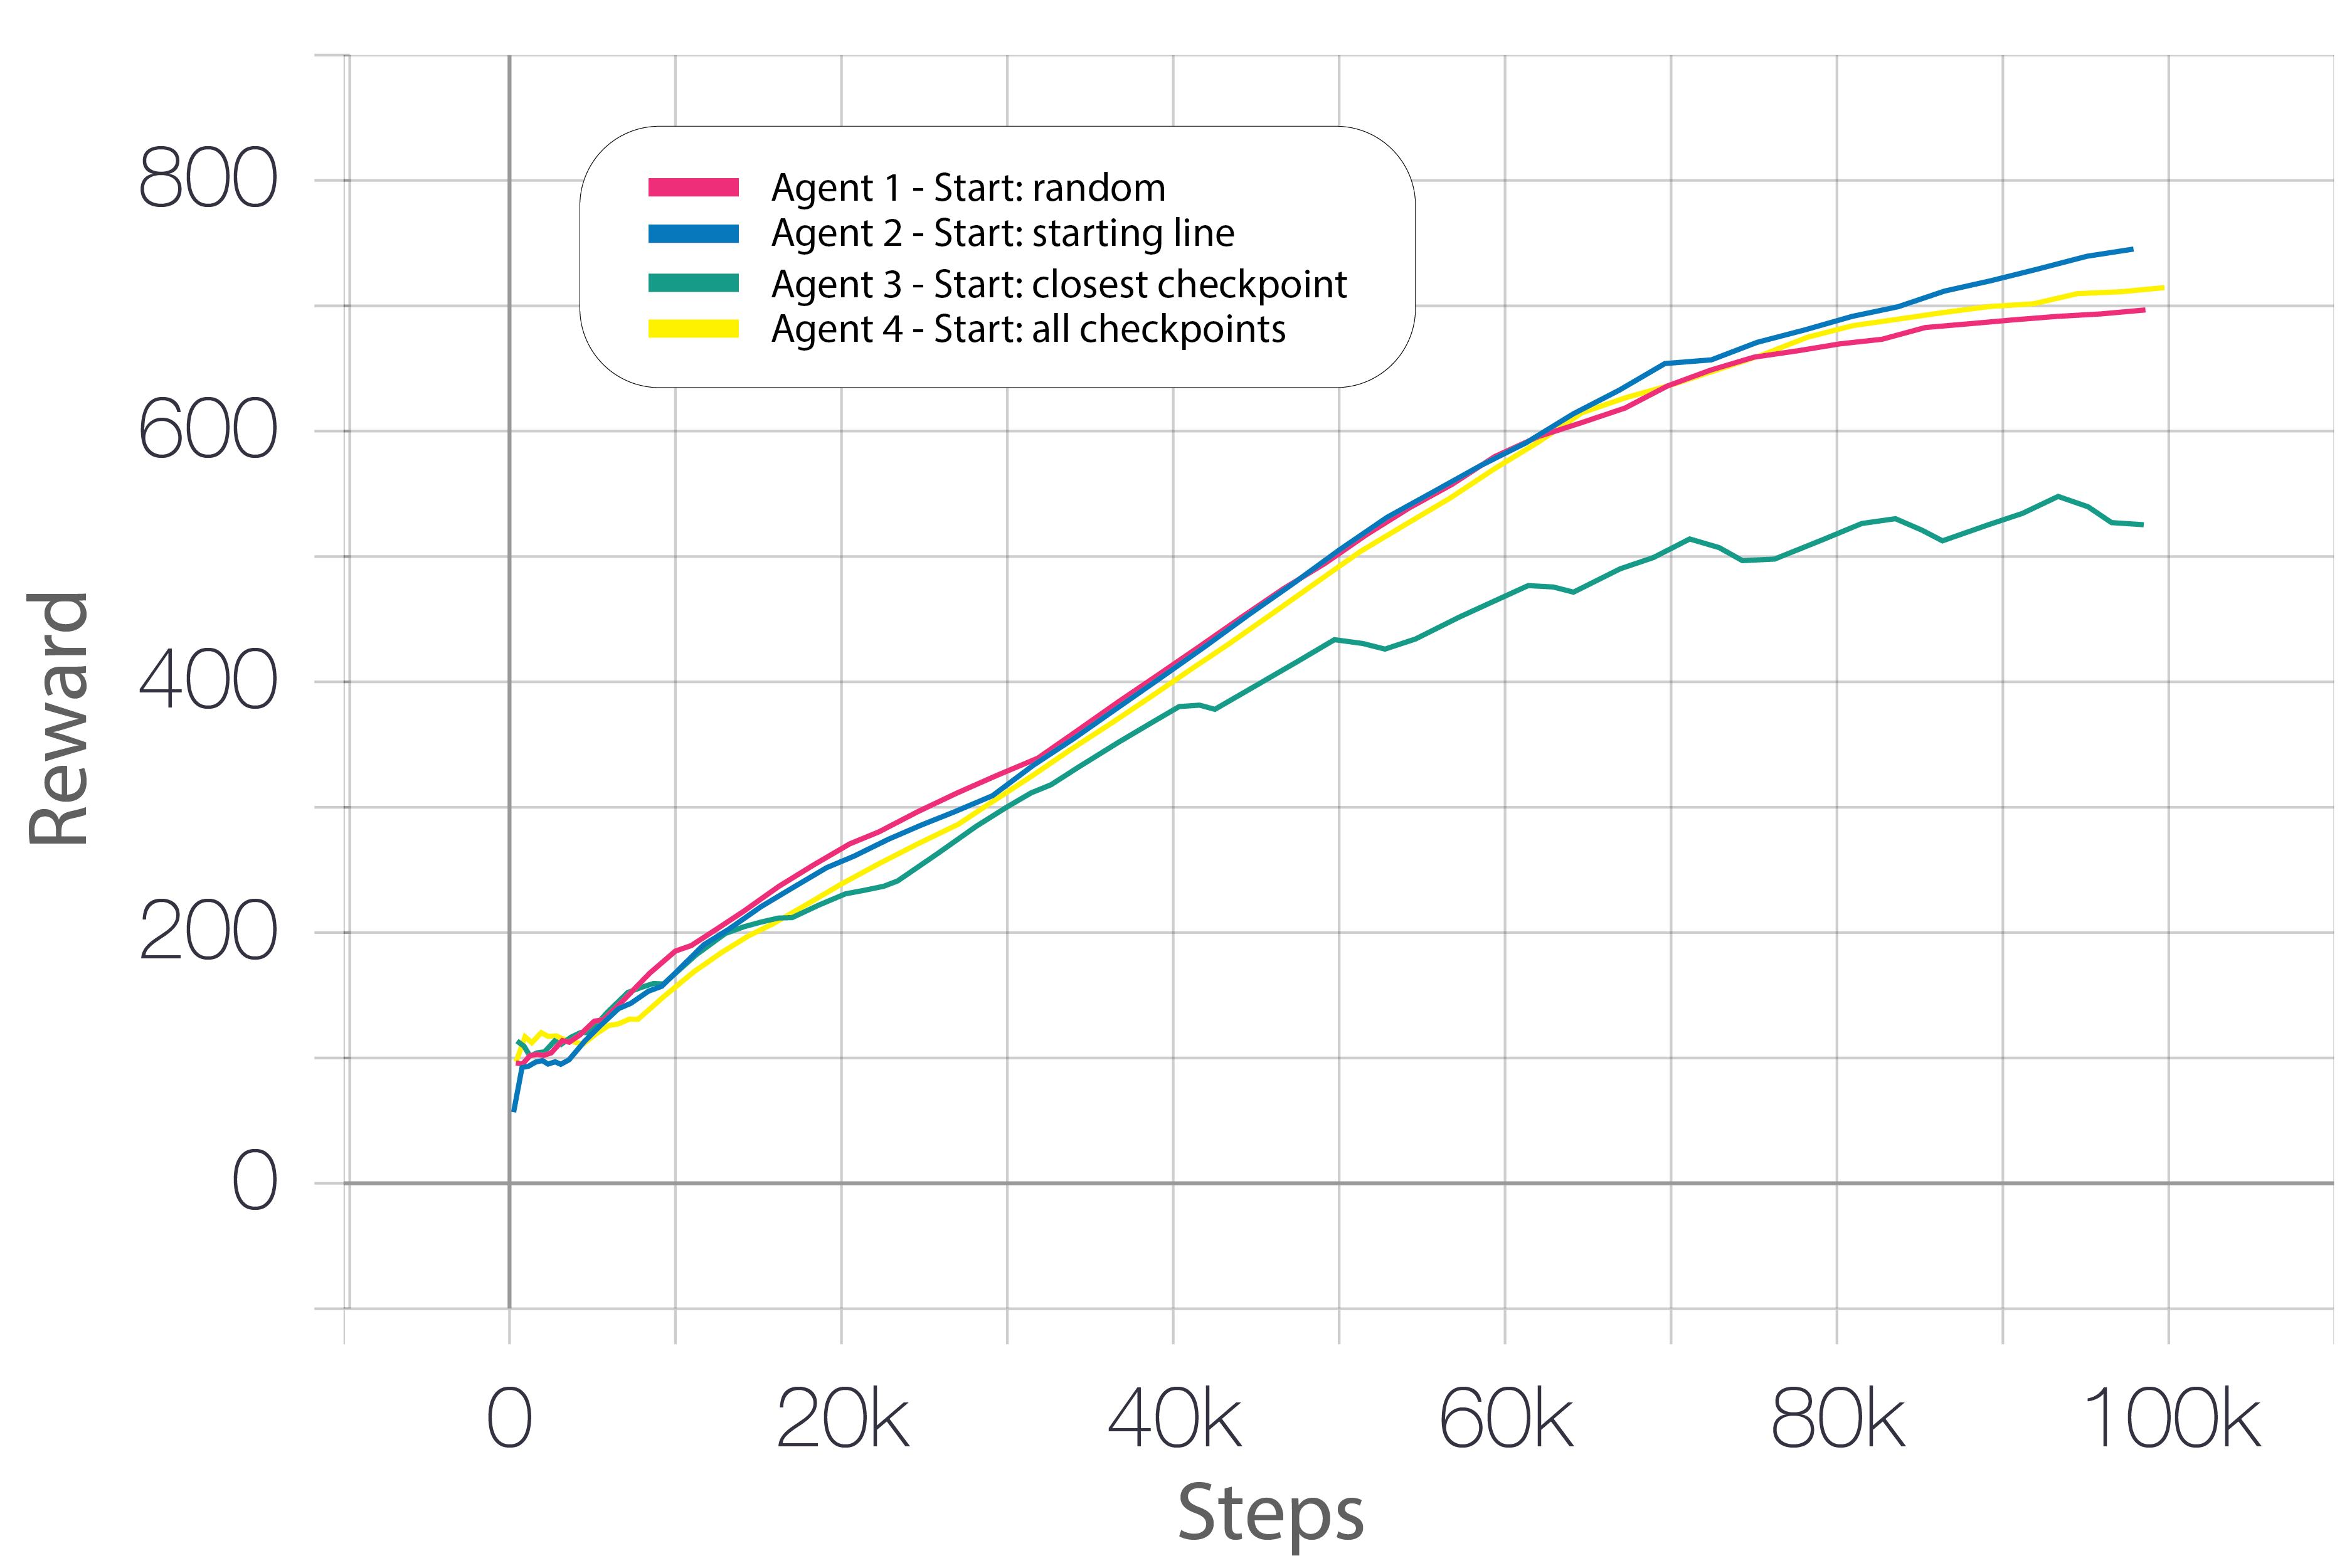
\includegraphics[width=1\textwidth]{experiments/rew_mean.png}
      \caption{Episodes reward mean}\label{fig:rew}
  \end{subfigure}
  
  \bigskip
  \begin{subfigure}{.45\linewidth}
    \centering
    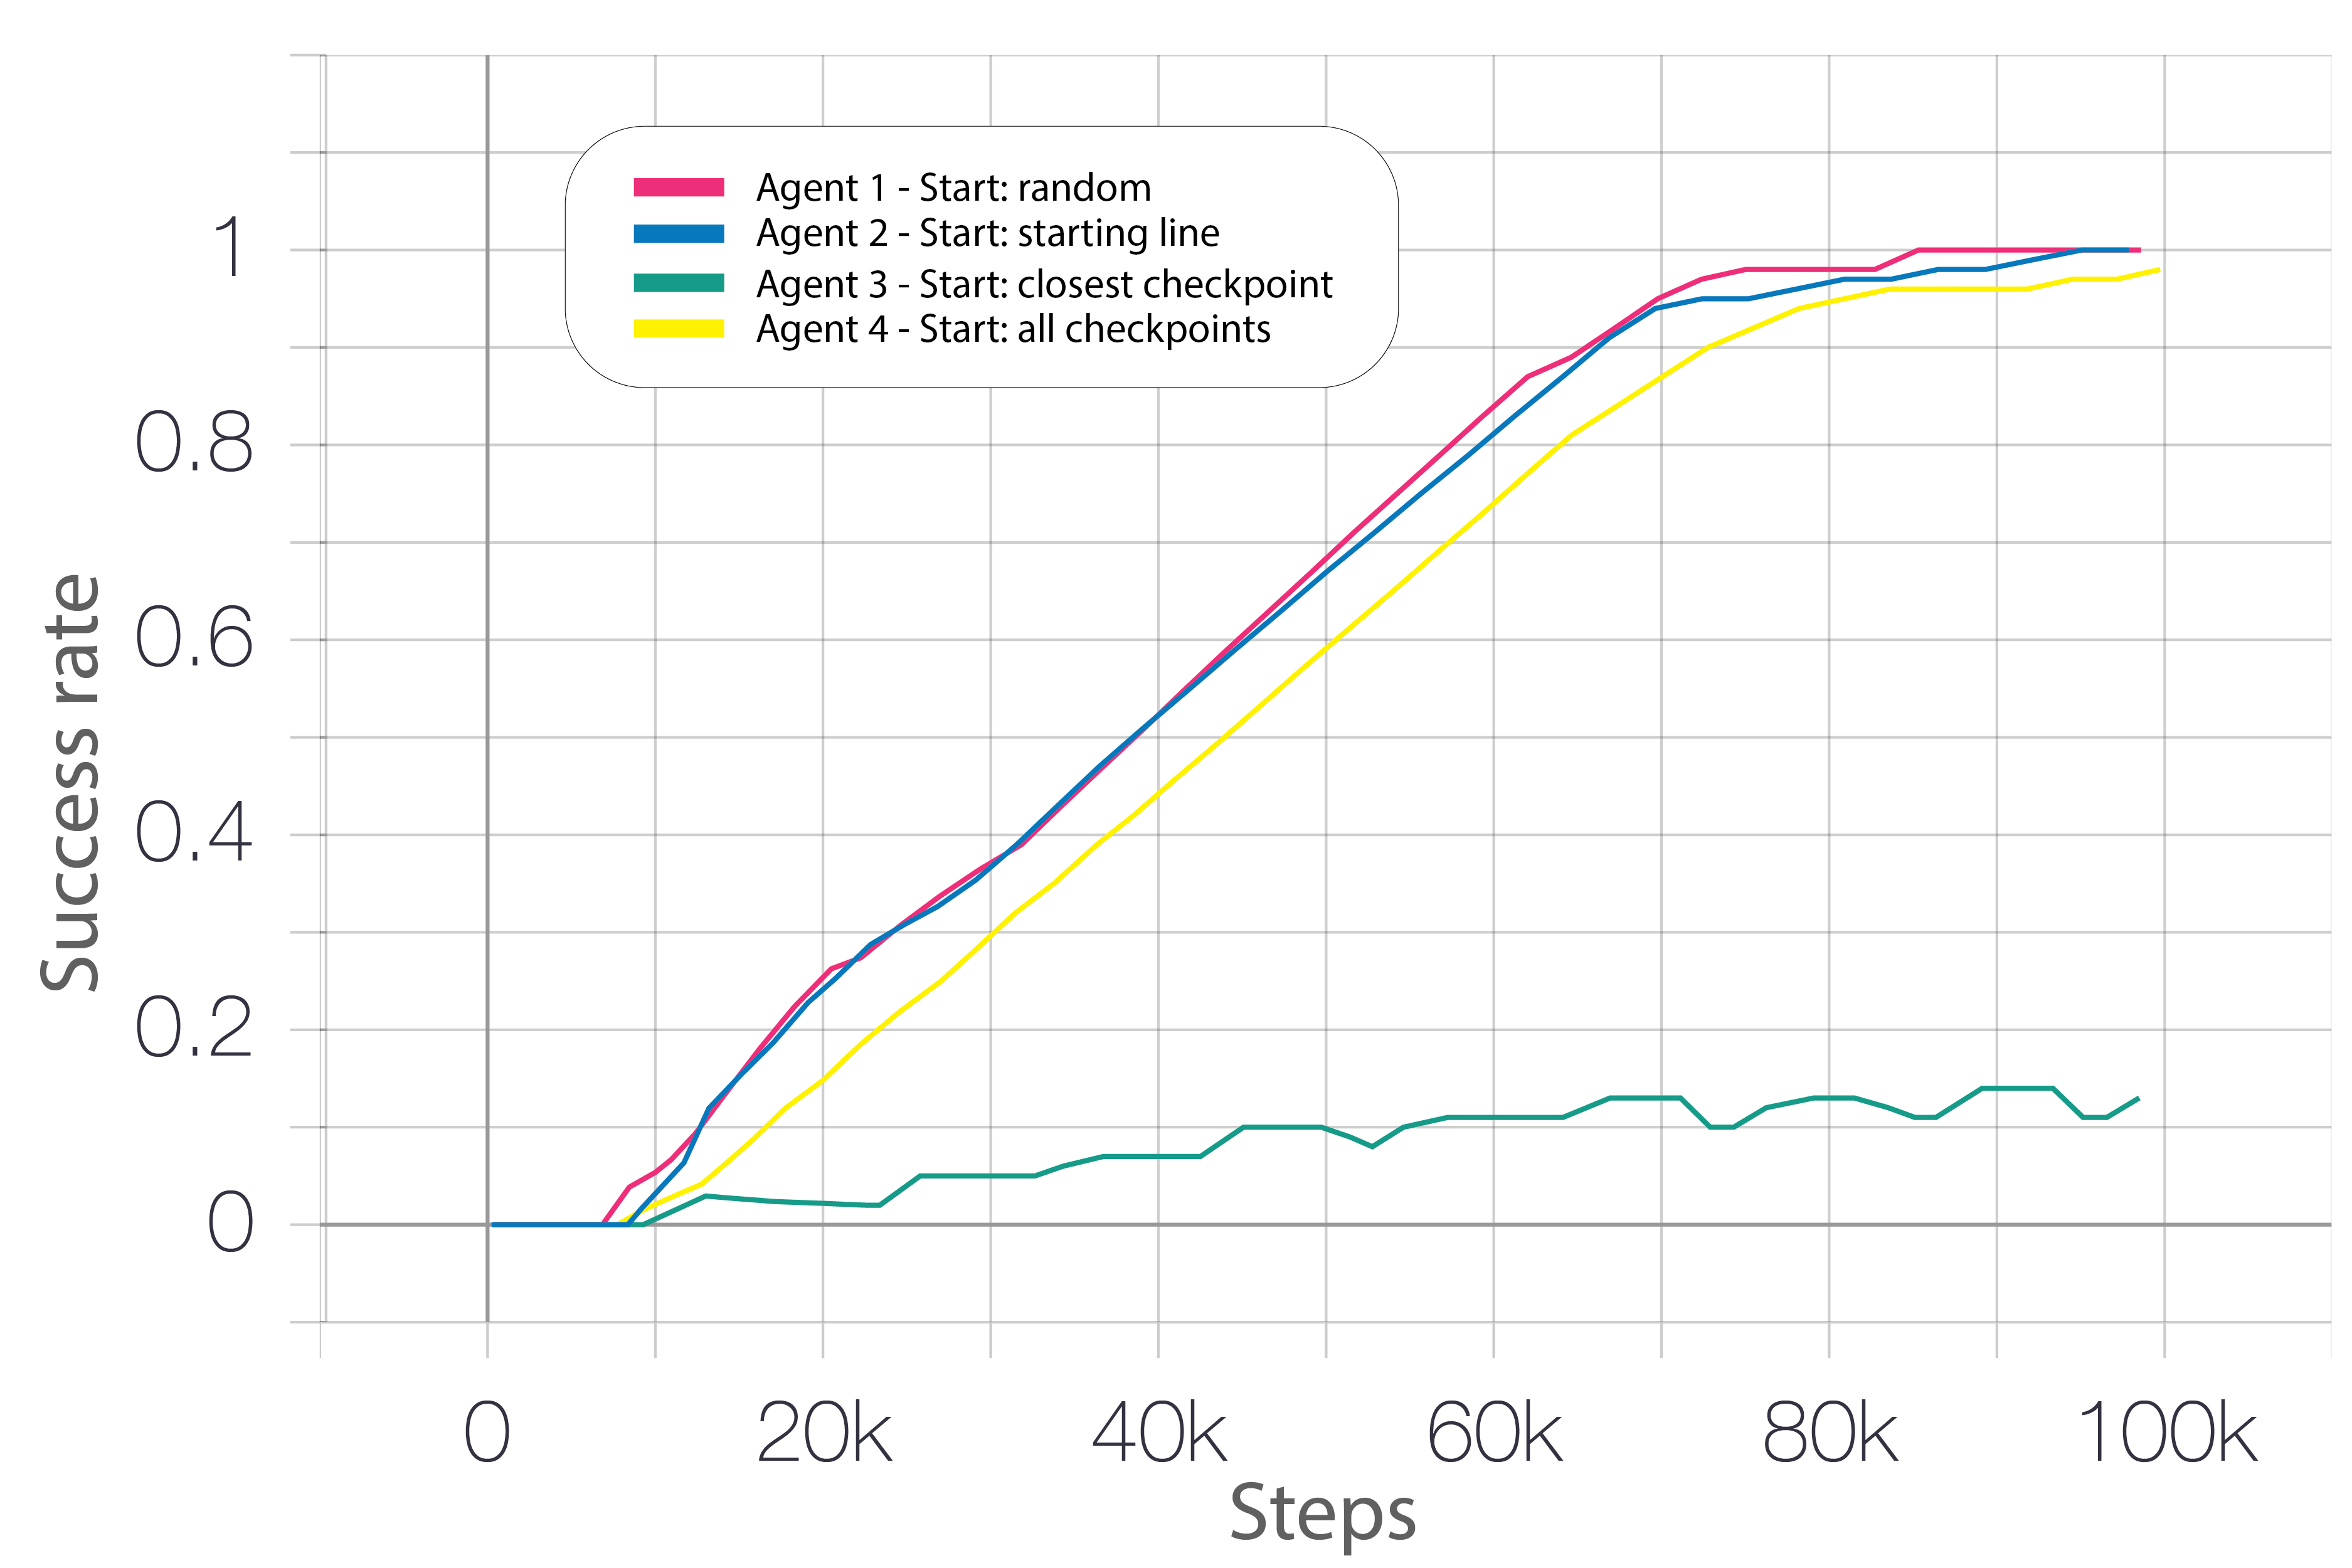
\includegraphics[width=1\textwidth]{experiments/success_mean.png}
    \caption{Success rate mean}\label{fig:succ}
  \end{subfigure} 
  \caption{Agents trained in simulation. Each agent has been trained with a different starting modality and has been trained for 100k steps.}
  \label{fig:agentresults}
\end{figure}
During our experiments, we noted that, in the best case, a lap may take $\approx 350$ iterations to be completed. The agents are all able to successfully learn to drive with a strict maximum CTE (3) except for \textit{Agent 4} which started new laps from the latest checkpoint. Two interesting shreds of evidence come out of those pieces of training. The first one is that even though the success rate mean approaches $100\%$, meaning the agents can consistently finish laps, the reward mean keeps growing. This shows a limitation in the reward function used, in fact, the agent gets a reward for every step and hence it learns to finish the lap following the longest path it has discovered. Moreover, the best way to lengthen the path is a zig-zag trajectory that allows also a doubling of the reward per lap. Secondly, the agent that starts at the latest checkpoint keeps improving the reward up to more than an equivalent completed lap, however, it never finishes a lap as described in Figure \ref{fig:succ}. The reason behind this strange behavior is that the agent found a bug in the simulator used, as shown in Figure \ref{fig:bug}. Essentially, there is a little spot, off track, close to the steepest turn where the CTE is not correctly detected by the simulator, and consequently, the episode is not terminated. The reason why this behavior only happened with this agent lies in the training modality. When the agent reaches that checkpoint, he cannot easily reach the next checkpoint given the toughness of the turn, instead, it finds it easier to explore the bugged spot which is almost right in front of it when it approaches the turn.

\begin{figure}[h]
  \begin{center}
    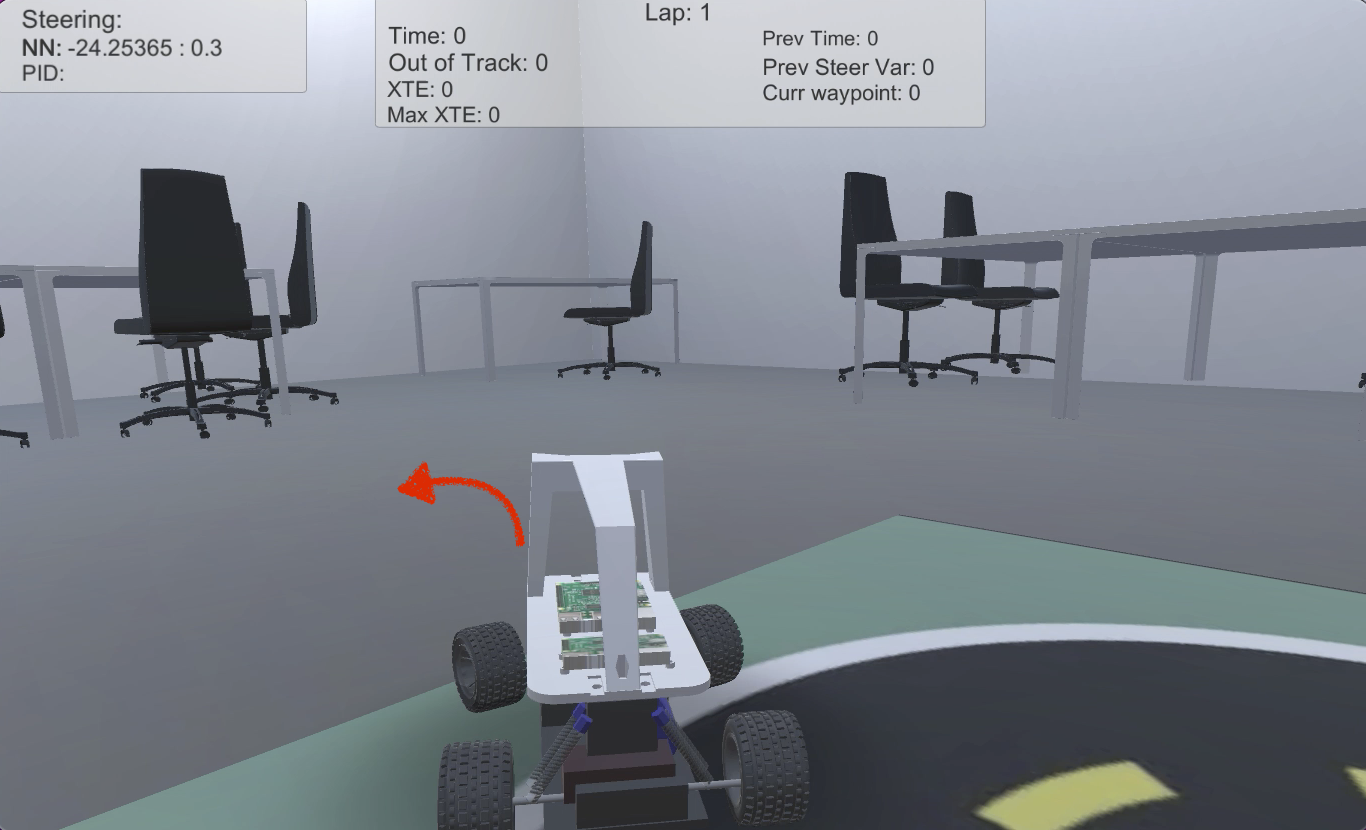
\includegraphics[width=0.50\textwidth]{experiments/bug.png}
  \end{center}
  \caption{Spotted bug in the simulator}
  \label{fig:bug}
\end{figure}

To further test the trained agents, for 10 laps it is measured how many times a lap has been completed by each agent, how many times the agents crash, and finally how many times they exceed the roadway but can recover and finish the lap without crashing. The result are presented in Table \ref{tab:simagent}.
\begin{table}
  \centering
  \begin{tabular}{|c|c|c|c|c|c|}
  \hline
  AGENT & OOT & OBE & LAPS & AVG LENGTH & AVG REW \\ \hline
  1 & 0 & 0 & 10 & 595 & 644 \\
  2 & 0 & 4 & 10 & 599 & 647  \\ \hline
  3 & 0 & 0 & 10 & 624 & 676 \\
  4 & 10 & 29 & 0 & 460 & 495  \\ \hline
  \end{tabular}
  \caption{Agents results averaged over 10 laps. Out Of Track (OOT) measures crashes, Out of Bound Error measure how many times it exceed the max CTE, and finally LAPS counts the completed laps.}
  \label{tab:simagent}
\end{table}
From the results is evident, excluding \textit{Agent 4} because of the simulator's bug, that three agents learned to successfully drive and in most cases, they always stay entirely on track without the need for any additional sensor and with the only problem of the shaky driving which is still acceptable for the purposes of this thesis, in most cases, they never get out of the track, and if they do they can recover consistently.

\subsection{Training the real RL agent}
To train the real-world agent, instead, the source code provided by \citet{learning-to-drive-in-5-minutes} is kept untouched beside the encoder, with the main goal being to replicate their results but with a more performing VAE as resulted in our tests. Given that in the real world the simulator's supervision is not available, all the strategies tested in the previous section are good candidates to be used, also \textit{Agent 4} strategy that cannot explore anymore the simulator's bug. In fact, in the real world, we only have human supervision that is about stopping the episode as soon as the car exceeds the track boundaries with all 4 wheels, while the server automatically stops the car when it reaches 1000 steps ($\approx 2.5$ laps). From the tests resulted that all the agents, trained with the aforementioned strategies, struggle to learn to drive an entire lap, at least in a reasonable time, except\textit{ Agent 4 }that start his laps at the latest checkpoint reached in the last episode. For the sake of brevity, since they are all equivalent among the failing agents, only the results of the agent that starts always at starting line and fails in learning, as shown in Figure \ref{fig:rlen}.

\begin{figure}[h]
  \centering
  \begin{subfigure}{.5\linewidth}
      \centering
      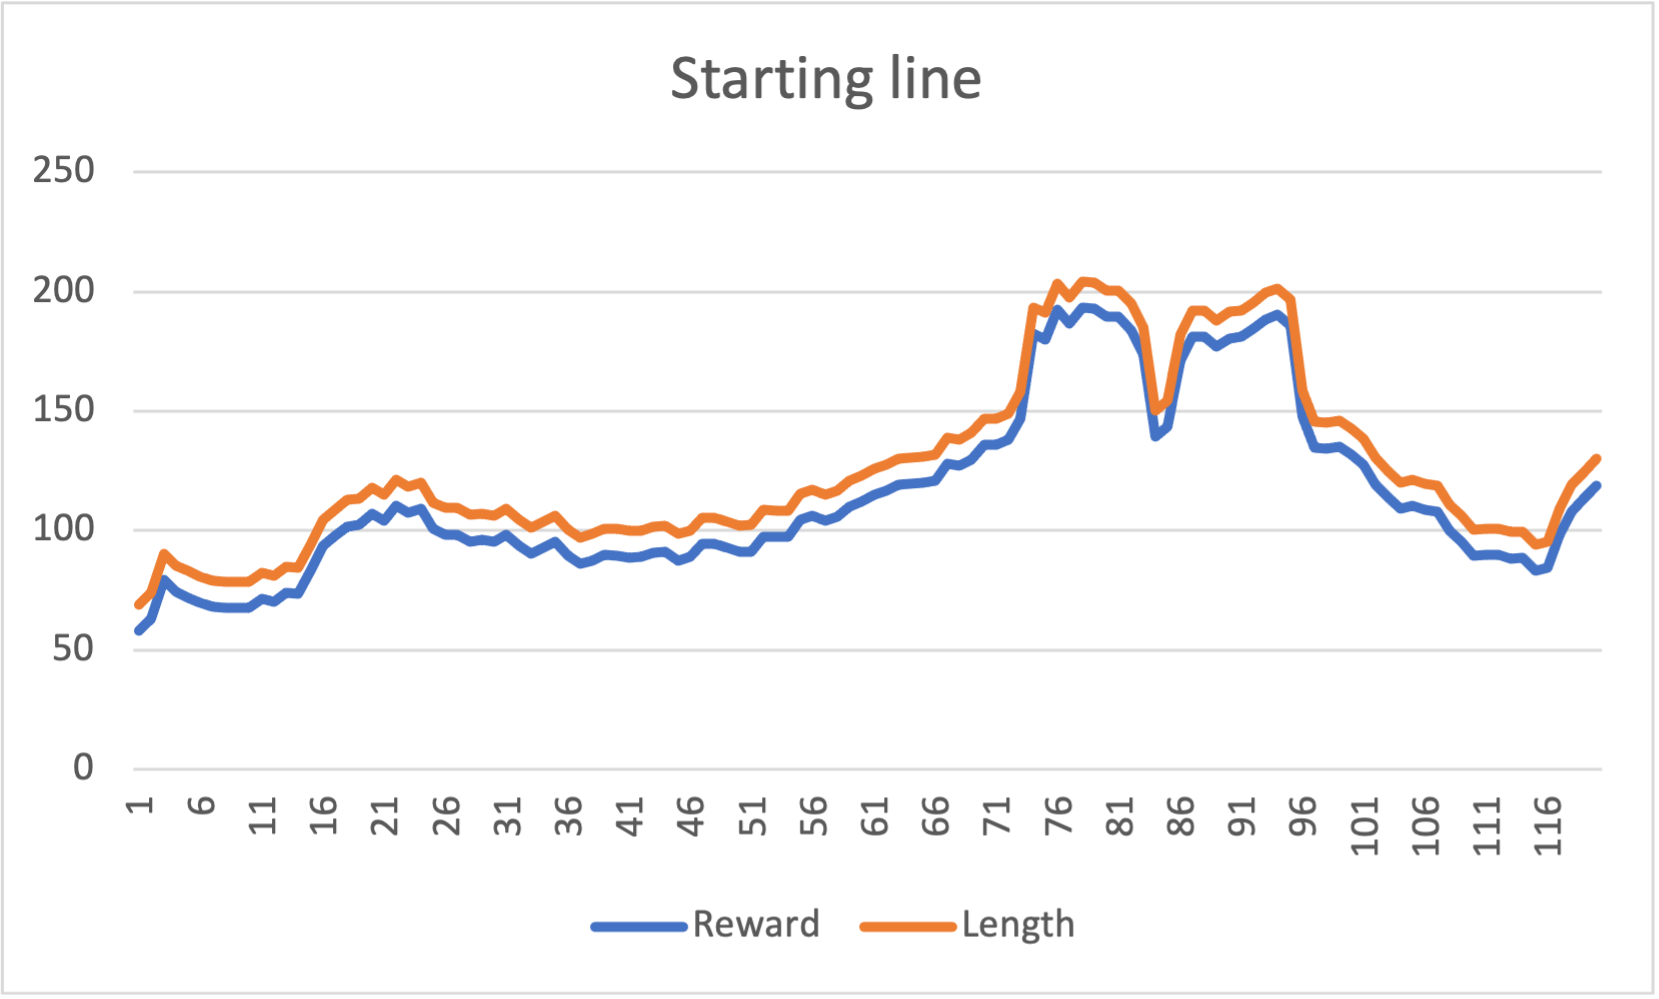
\includegraphics[width=1\textwidth]{experiments/badrealagentstart.png}
      \caption{Agent performances: starting line}\label{fig:rlen}
  \end{subfigure}%
      \hfill
  \begin{subfigure}{.5\linewidth}
      \centering
      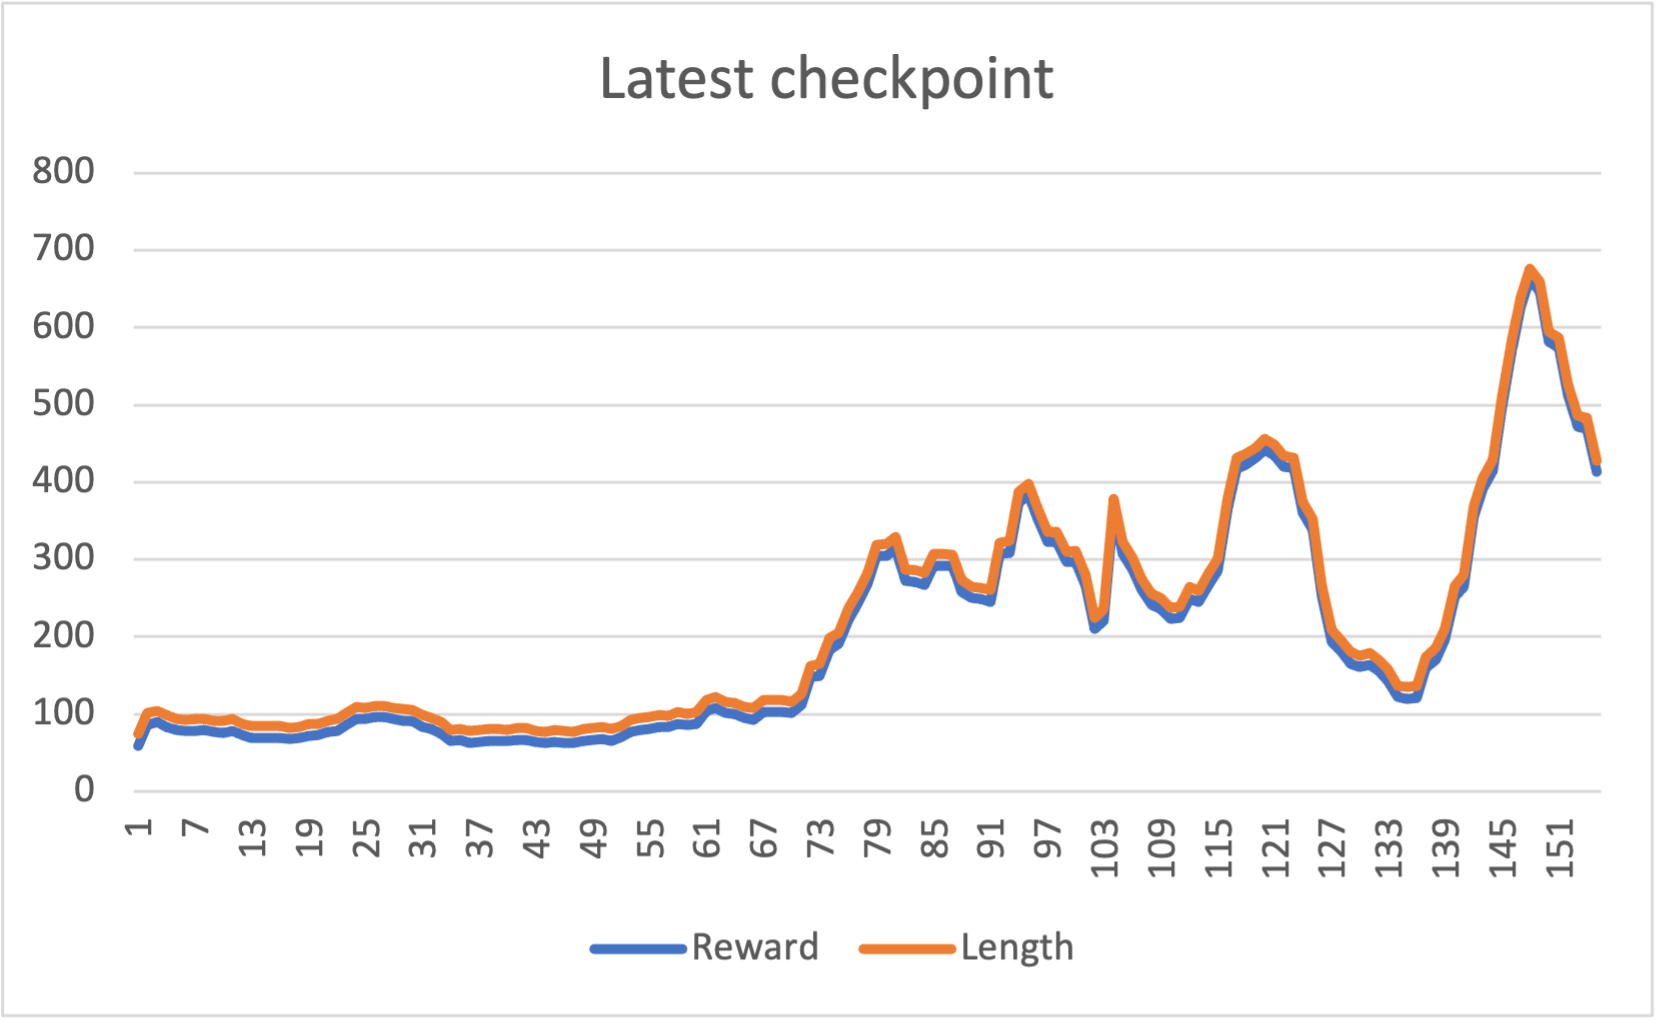
\includegraphics[width=1\textwidth]{experiments/badrealagentlatest.png}
      \caption{Agent performances: latest checkpoint}\label{fig:rrew}
  \end{subfigure}
  \caption{Agent trained in real world starting each lap at the starting line on the left and agent starting at the latest checkpoint on the right}
  \label{fig:realresult}
\end{figure}

In figure \ref{fig:rrew}, instead, are shown the performances in the training of the agent starting at the latest checkpoint (equivalent strategy of previous \textit{Agent 4}), which can be considered successful and comparable to simulated agents since it did learn to complete a lap in about 30 minutes and two laps in about 45 minutes. In five to twenty episodes, the first two turns were learned decently and most of the time was spent on the steepest turn. As shown in Figure \ref{fig:rlen}, the graph is characterized by ups and downs, as soon as the car started at the starting line, it learned quickly, then, when the steepest curve was reached it struggled to overcome it and when it eventually did, the length started to increase again. The process was repeated until it was almost consistently able to finish a lap. Furthermore, as soon as the agent learned the steepest turn, it did generalize well on the following turns and little time was spent on them.

Notice that the laying of the car at the latest checkpoint has been intentionally approximate on the area close to the checkpoints. This brought a main advantage, the agent learned quicker since it was able to see the area in front of it from many points of view and this, resulted useful when the car started to cross many checkpoints per episode since the direction from which the car arrived to a checkpoint could vary a lot, it had been trained to drive on many possible trajectories and was able to join the various sections well. Unfortunately, in the real world, more metrics to measure the quality of the driving and to make comparisons with the simulated agents are not available.

A major problem that arose from the training was the DonkeyCar slowly decreasing his speed during episodes even though the throttle was kept constant. From on point of view we could see how a slower speed helped in driving, however changing the speed uncontrollably define training procedures that are not easily replicable. To minimize the problem we noted that unplugging the battery for a moment, once in a while, would restore the full speed of the car, that is why we suspect the problem was given by the battery and so can be easily fixed.

\section{Sim to Real}

In this section we present an unsuccessful attempt in driving our simulated DonkeyCar with the real agent trained above. SimToReal (S2R) and vice-versa aims in deploying model trained in one environment to the other. In our case, since the real world environment, in our setup, does not provide enough metrics to benchmark our real world agent, we aim to make it works also in simulation. For example, in order to test the generalization of the real agent would be much easier in simulation where multiple tracks or obstacles can be implemented at a low cost. Another advantage brought by this approach is that an agent trained in simulation, can be moved into the real world and this would result in less expensive training procedures and eventually more robust agents. The idea is to pre-train a CycleGan \citep{CycleGAN2017} for image transfiguration. In fact, the CycleGan is able to move an image into another domain keeping the original structure unaltered, but applying the style of the other domain as shown in Figure \ref{fig:cycleganexample}. Thus we leverage this property to transform images seen by the simulated camera of the DonkeyCar into what it would see in real world and vice-versa. Then, a real agent will eventually be able to drive on the simulator since it does see pseudo-real images. On the other hand, in order to drive a real car with a simulated agent, our DonkeyCar has not enough computational power, hence it could not run in time a CycleGan, that has millions of parameters, to make the real car see pseudo-simulated images and drive with the simulated agent. However, the problem can be circumvented by training an agent entirely on simulation but with pseudo-real images. After training CycleGAN with our datasets, it is able to transfigure image with high fidelity as shown in Figure \ref{fig:cycleganexample}. In fact, in human eyes they are barely distinguishable. However, even if the result looks good it could not be the case for the AutoEncoder that needs to place similar real and pseudo real images close into the latent space and similarly for similar simulated and pseudo simulated images.

\begin{figure}[h]
  \centering
  \begin{subfigure}{.6\linewidth}
      \centering
      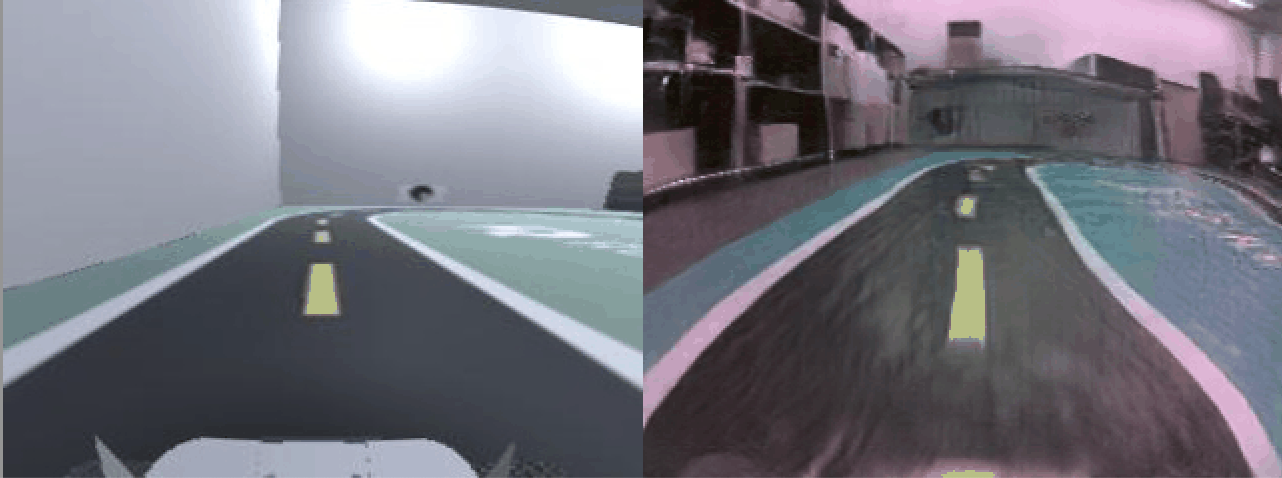
\includegraphics[width=1\textwidth]{experiments/s2r.png}
      \caption{From simulated images to pseudo-real}\label{fig:s2r}
  \end{subfigure}
      \hfill
  \begin{subfigure}{.6\linewidth}
      \centering
      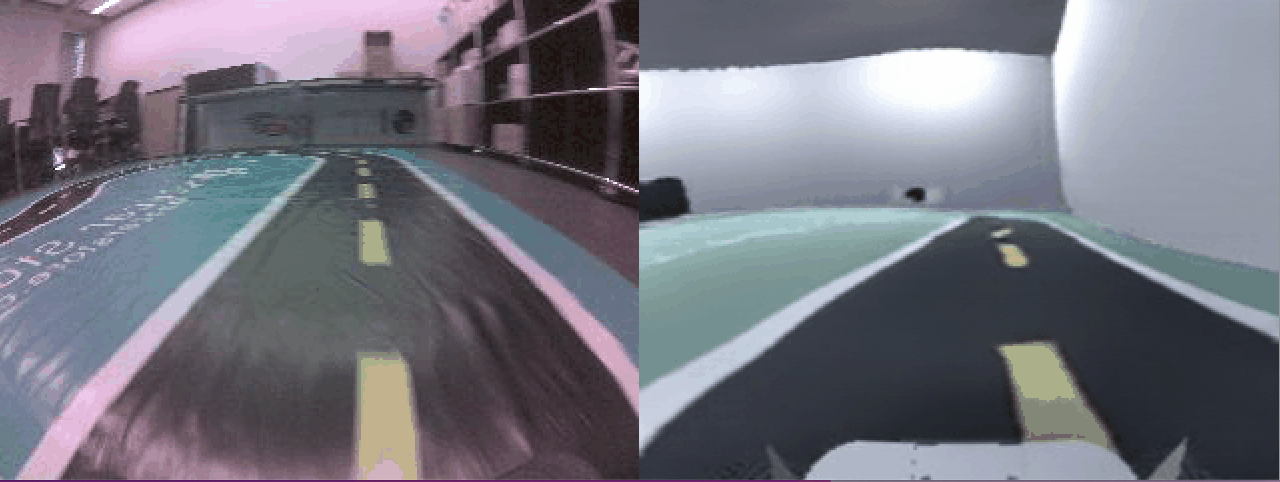
\includegraphics[width=1\textwidth]{experiments/r2s.png}
      \caption{From real images to pseudo-simulated}\label{fig:r2s}
  \end{subfigure}
  \caption{CycleGAN capabilities after training on our dataset}
  \label{fig:cycleganexample}
\end{figure}
Hence, the real test set is transformed through the CycleGAN and then forwarded through the real VAE chosen and similarly for the simulated test set. Given that 64 dimension cannot be visualized, a further dimensionality reduction is applied with t-SNE down to two dimension, as shown in Figure \ref{fig:latentpseudo}.
\begin{figure}[h]
  \centering
  \begin{subfigure}{.5\linewidth}
      \centering
      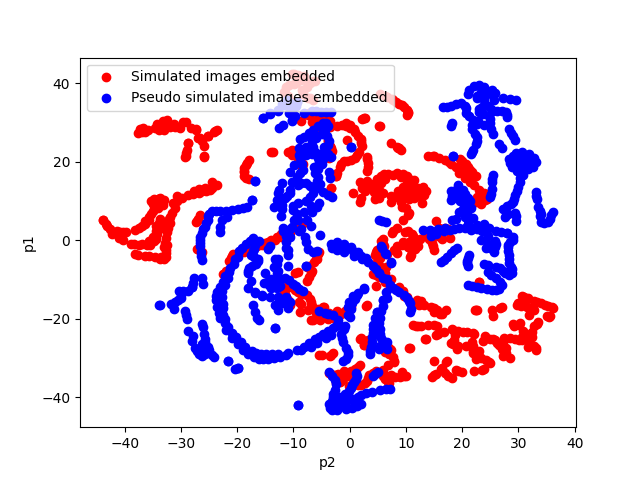
\includegraphics[width=1\textwidth]{experiments/latentr2s.png}
      \caption{Simulated and pseudo simulated images}\label{fig:latentr2s}
  \end{subfigure}%
      \hfill
  \begin{subfigure}{.5\linewidth}
      \centering
      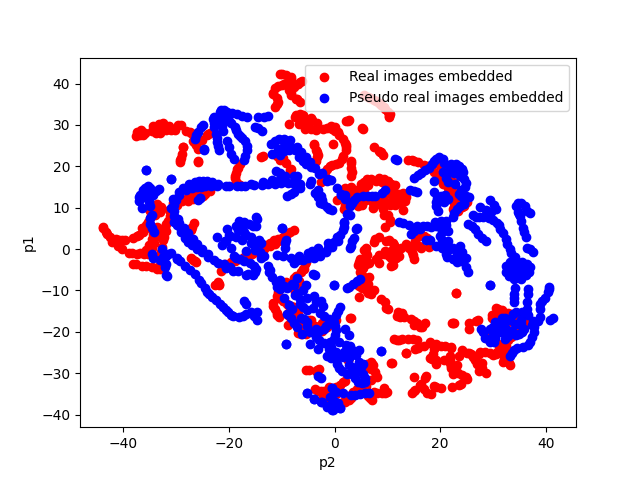
\includegraphics[width=1\textwidth]{experiments/latents2r.png}
      \caption{Real and pseudo real images}\label{fig:latents2r}
  \end{subfigure}
  \caption{Images embedded into the latent space with respectively the simulated and the real VAE.}
  \label{fig:latentpseudo}
\end{figure}
Since the datasets are not aligned we do not except a perfect overlap, instead, the encoder should be able to at least embed similar images in the same region of the space. However, the latent space shows that is not always the case, some regions does overlap but not all off them in both real and simulated dataset. This could lead the trained agent not to respond consistently in similar situations. A further attempt is made by aligning the set of data used through the CycleGAN. Once the CycleGAN has been used to transform simulated images into pseudo real images, it can be used again to bring them back to pseudo simulated images, resulting in aligned sets. However, notice that the distortion, barely visible before, increases as shown in Figure \ref{fig:examplealigned}.
\begin{figure}[h]
  \centering
  \begin{subfigure}{.33\linewidth}
      \centering
      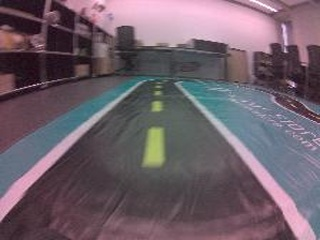
\includegraphics[width=1\textwidth]{experiments/0_.jpg}
      \caption{Real image}\label{fig:real}
  \end{subfigure}%
      \hfill
  \begin{subfigure}{.33\linewidth}
      \centering
      \scalebox{-1}[1]{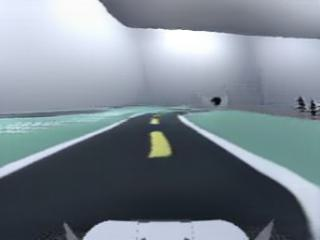
\includegraphics[width=1\textwidth]{experiments/0__.jpg}}
      \caption{Pseudo simulated image}\label{fig:psim}
  \end{subfigure}%
  \hfill
  \begin{subfigure}{.33\linewidth}
    \centering
    \scalebox{-1}[1]{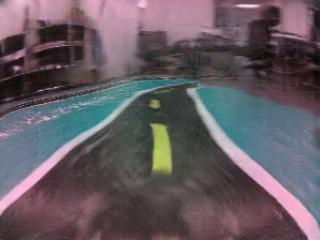
\includegraphics[width=1\textwidth]{experiments/0___.jpg}}
    \caption{Pseudo pseudo real}\label{fig:ppreal}
  \end{subfigure} 
  \caption{Example of using the CycleGan to create an aligned dateset}
  \label{fig:examplealigned}
\end{figure}

\begin{figure}[h]
  \centering
  \begin{subfigure}{.5\linewidth}
      \centering
      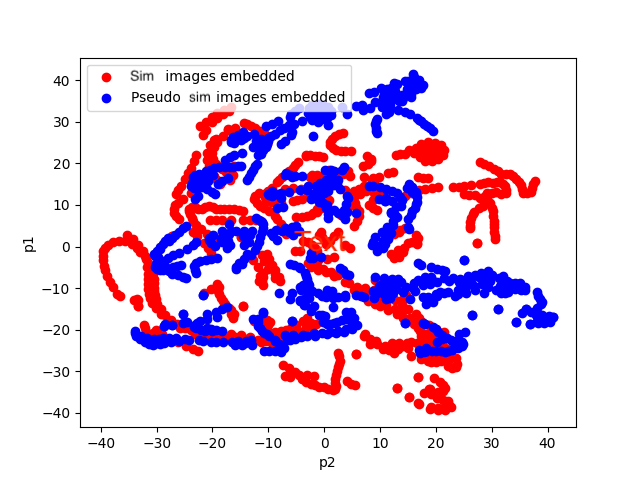
\includegraphics[width=1\textwidth]{experiments/aligned_latentr2s.png}
      \caption{Aligned simulated and pseudo sim images}\label{fig:aligen_latentr2s}
  \end{subfigure}%
      \hfill
  \begin{subfigure}{.5\linewidth}
      \centering
      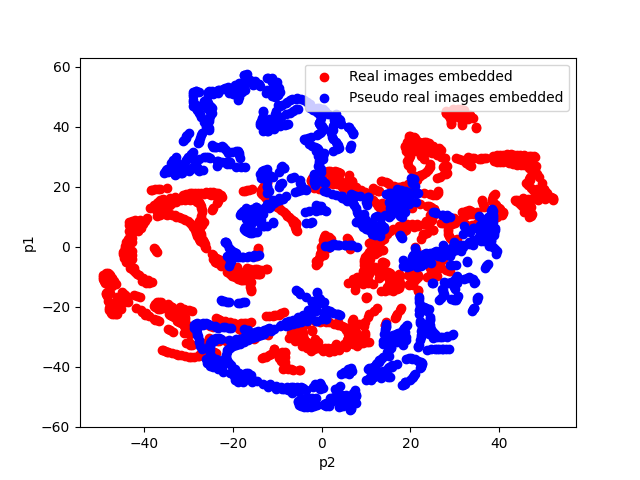
\includegraphics[width=1\textwidth]{experiments/aligned_latents2r.png}
      \caption{Aligned real and pseudo real images}\label{fig:aligen_latents2r}
  \end{subfigure}
  \caption{Aligned images embedded into the latent space with respectively the simulated and the real VAE.}
  \label{fig:latentpseudoaligned}
\end{figure}
Unfortunately, the results do not change enough from the previous one as shown in Figure \ref{fig:latentpseudoaligned}. Given that the t-SNEe dimensionality reduction may be a cause of our problem, a further investigation is made by checking what are the closest images between the real set and pseudo real set and similarly for the simulated set in the latent space. The distance measure used is the Euclidean distance and by looking at them there is some problem, in fact there are perfect matches as well as wrong matches as shown in Figures \ref{fig:simdistance} and \ref{fig:realdistance}. This may be the cause of our agent not being able to drive when transferred into another domain, the encoder is not robust enough to compensate little image distortion.

As a final test, we are interested in studying what would be the actions undertaken by the agent on a set of aligned pictures. In particular, we selected a small set of 100 contiguous real pictures of the track and created its \textit{aligned} pseudo real version. We then checked what would be the action of the real agent. As shown in Figure \ref{fig:path_rec}, the results are interesting since most of the times the agent takes a similar action on both images, however even a tiny difference can lead the car out of track from which often it is not able to recover in time and the simulator ends the lap. The mean error on the predicted action resulted to be 0.205 with a standard deviation of 0.183. In conclusion, even a small mean error does not let the agent drives in a different environment than the one in which it was trained, hence this procedure is too premature to be effective and needs further studies, especially in the latent space alignment between real and pseudo real images. However, the ease with which these results have been obtained bodes well.

\begin{figure}[h]
  \begin{center}
    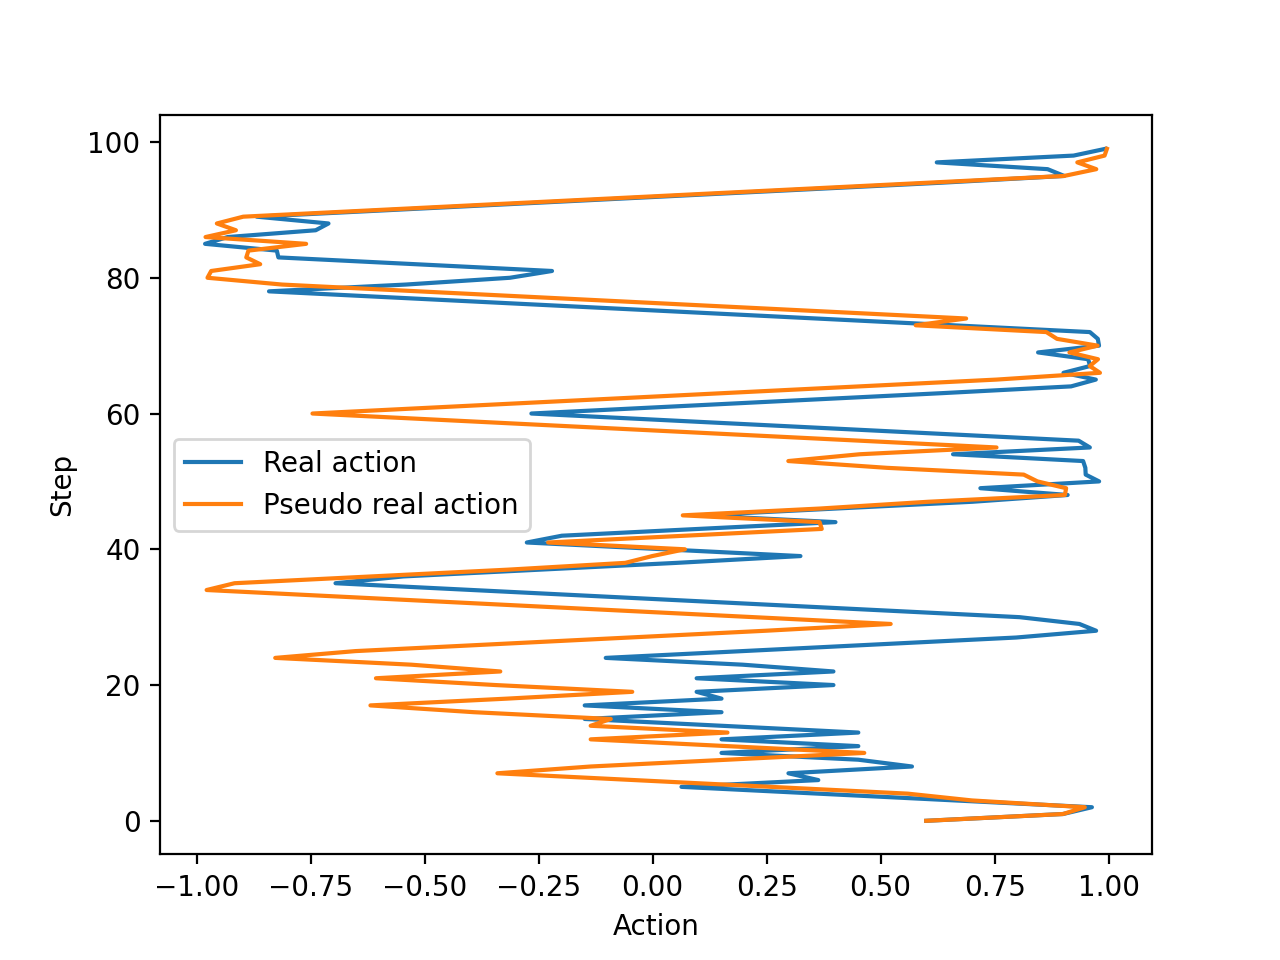
\includegraphics[width=0.60\textwidth]{experiments/path_rec.png}
  \end{center}
  \caption{Real agent's actions on an aligned dataset}
  \label{fig:path_rec}
\end{figure}

\begin{figure}[h]
  \centering
  \begin{subfigure}{.24\linewidth}
      \centering
      \scalebox{-1}[1]{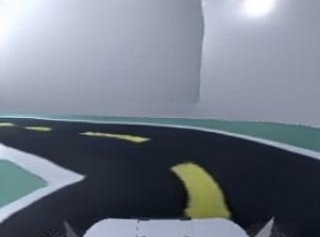
\includegraphics[width=1\textwidth]{experiments/badsimdist1.jpg}}
      \caption{Pseudo simulated}\label{fig:badsimdist1}
  \end{subfigure}%
  \hfill
  \begin{subfigure}{.24\linewidth}
    \centering
    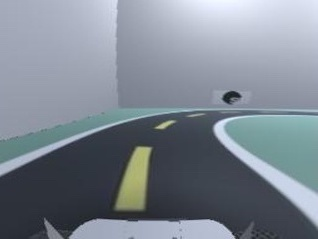
\includegraphics[width=1\textwidth]{experiments/badsimdist2.jpg}
    \caption{Closest simulated}\label{fig:badsimdist2}
  \end{subfigure}%
  \hfill
  \begin{subfigure}{.24\linewidth}
      \centering
      \scalebox{-1}[1]{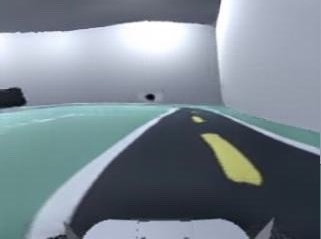
\includegraphics[width=1\textwidth]{experiments/goodsimdist1.jpg}}
      \caption{Pseudo simulated}\label{fig:goodsimdist1}
  \end{subfigure}%
  \hfill
  \begin{subfigure}{.24\linewidth}
    \centering
    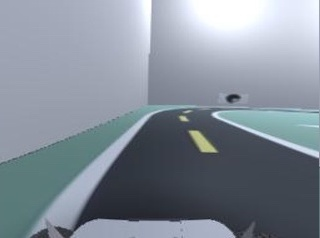
\includegraphics[width=1\textwidth]{experiments/goodsimdist2.jpg}
    \caption{Closest simulated}\label{fig:goodsimdist2}
\end{subfigure}
  \caption{Figures \ref{fig:badsimdist1} and \ref{fig:goodsimdist1} show two pseudo simulated images and Figures \ref{fig:badsimdist2} and \ref{fig:goodsimdist2} respectively the closest match in the simulated set measured with the Euclidean Distance.}
  \label{fig:simdistance}
\end{figure}

\begin{figure}[h]
  \centering
  \begin{subfigure}{.24\linewidth}
      \centering
      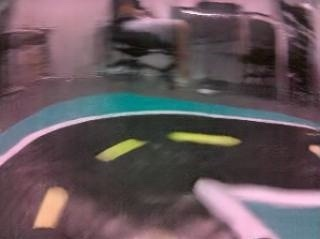
\includegraphics[width=1\textwidth]{experiments/badrealreal1.jpg}
      \caption{Pseudo real}\label{fig:badrealdist1}
  \end{subfigure}%
  \hfill
  \begin{subfigure}{.24\linewidth}
    \centering
    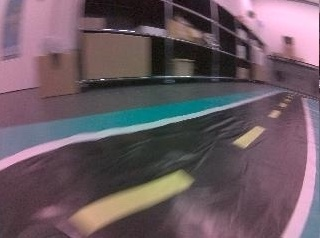
\includegraphics[width=1\textwidth]{experiments/badrealreal2.jpg}
    \caption{Closest real}\label{fig:badrealdist2}
  \end{subfigure}%
  \hfill
  \begin{subfigure}{.24\linewidth}
      \centering
      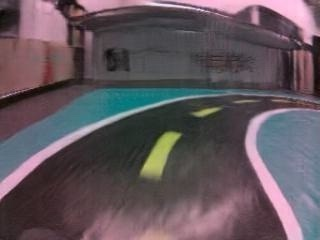
\includegraphics[width=1\textwidth]{experiments/goodrealdist1.jpg}
      \caption{Pseudo real}\label{fig:goodrealdist1}
  \end{subfigure}%
  \hfill
  \begin{subfigure}{.24\linewidth}
    \centering
    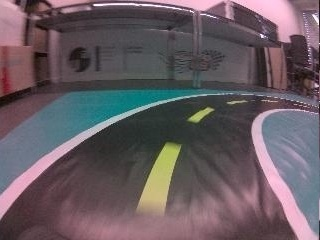
\includegraphics[width=1\textwidth]{experiments/goodrealdist2.jpg}
    \caption{Closest real}\label{fig:goodrealdist2}
\end{subfigure}
  \caption{Figures \ref{fig:badrealdist1} and \ref{fig:goodrealdist1} show two pseudo real images and Figures \ref{fig:badrealdist2} and \ref{fig:goodrealdist2} respectively the closest match in the real set measured with the Euclidean Distance.}
  \label{fig:realdistance}
\end{figure}



